\section{Port System}
\label{sec:impl_port_system}

This section describes the typed and unit-aware port system used by all \texttt{CoSimComponent} instances.
It realizes \ref{req:SR-01-01} under \ref{req:UR-01} and \ref{req:SR-02-01}--\ref{req:SR-02-03} under \ref{req:UR-02}.
The implementation provides the port interface introduced in Section~\ref{sec:architecture_cosimcomponent}.
The same machinery supports connection validation, value propagation, history recording, and event-port creation.

%%%%%%%%%%%%%%%%%%%%%%%%%%%%%%%%%%%%%%%%%%%%%%%%%%%%%%
\subsection{Specification and State}

The implementation separates the static port specification from the mutable runtime value, as shown in Figure~\ref{fig:impl_port_system}.
The \texttt{PortSpec} class defines the interface contract of a port.
The \texttt{PortState} class stores the current value and validates every runtime update against this contract.

\begin{figure}[htbp]
  \centering
  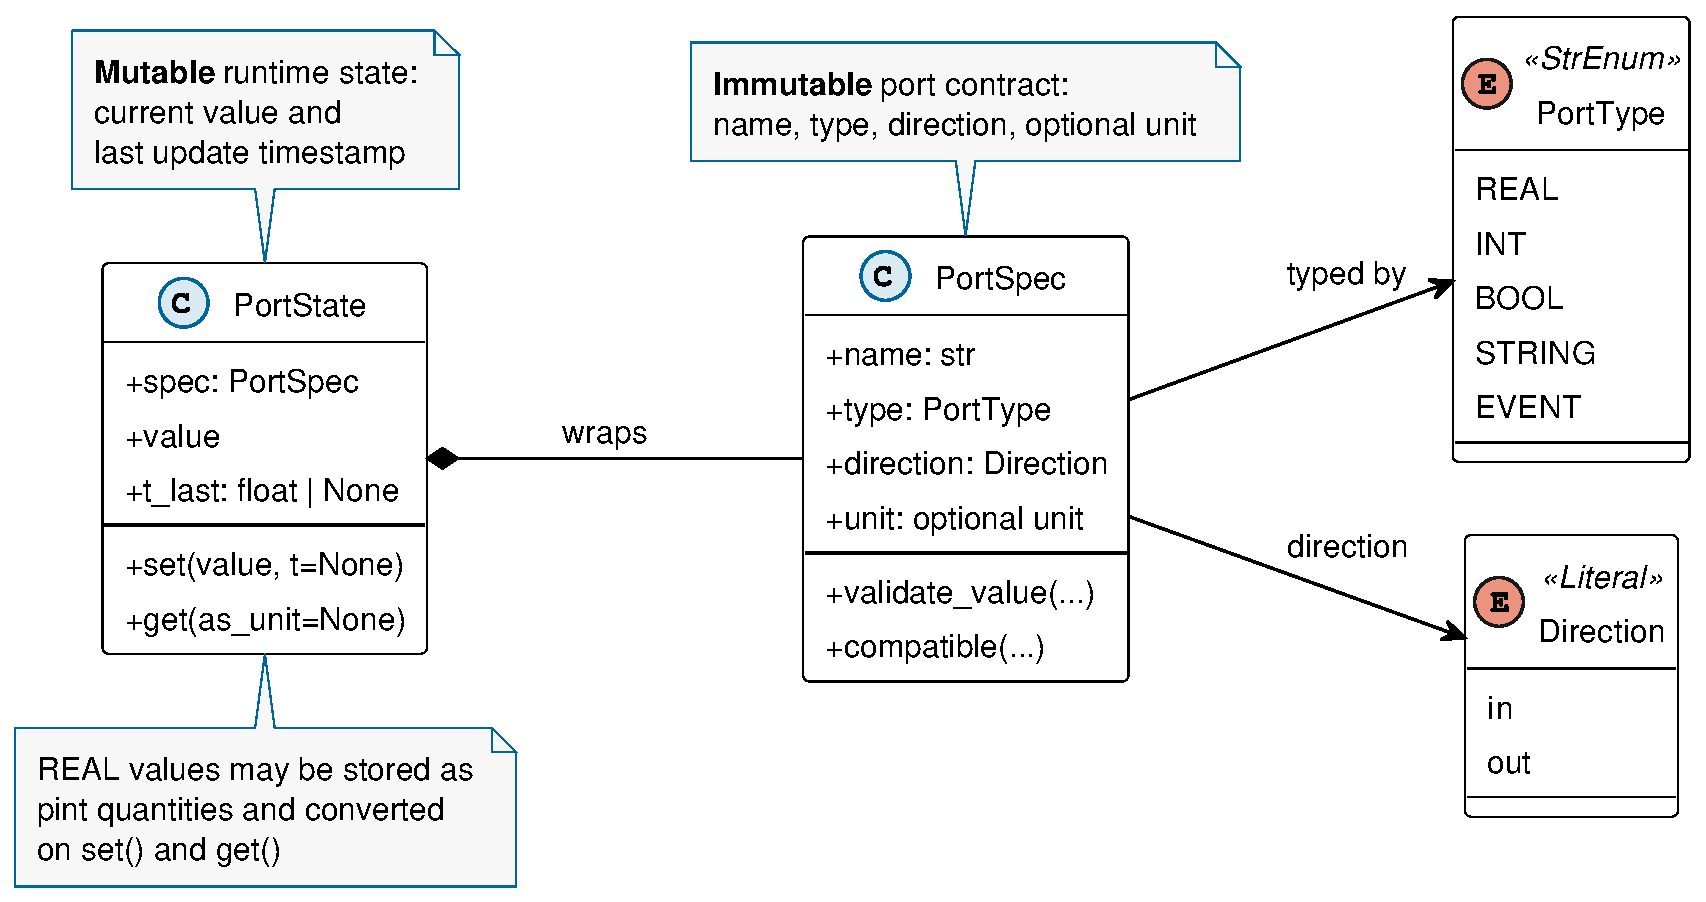
\includegraphics[width=0.75\linewidth]{diagrams/out/pdf/class/core/Port.pdf}
  \caption[Class diagram of the port system]{Class diagram of the port system.
  The \texttt{PortSpec} class defines the immutable port contract.
  The \texttt{PortState} class stores the runtime value and applies type and unit validation.}
  \label{fig:impl_port_system}
\end{figure}

\paragraph{Port Types.}
Table~\ref{tab:impl_port_types} lists the supported data types.
They are implemented by the \texttt{PortType} enumeration.
Physical units are allowed only for \texttt{REAL} ports.
The \texttt{EVENT} type represents boolean trigger ports.
Such ports are created automatically for registered event indicators during component initialization, as described in Section~\ref{sec:impl_component_interface}.

\begin{table}[htbp]
  \centering
  \small
  \caption{Supported port data types in the \texttt{PortType} enumeration.}
  \label{tab:impl_port_types}
  \begin{tabular}{lll}
    \toprule
    \textbf{Type}   & \textbf{Python value}                    & \textbf{Unit allowed} \\
    \midrule
    \texttt{REAL}   & \texttt{float} or \texttt{pint.Quantity} & yes                   \\
    \texttt{INT}    & \texttt{int}                             & no                    \\
    \texttt{BOOL}   & \texttt{bool}                            & no                    \\
    \texttt{STRING} & \texttt{str}                             & no                    \\
    \texttt{EVENT}  & \texttt{bool} (trigger)                  & no                    \\
    \bottomrule
  \end{tabular}
\end{table}

\paragraph{Port Specification.}
A \texttt{PortSpec} is a frozen dataclass that describes one port.
It stores the port name, direction, data type, optional physical unit, and an optional description.
Unit strings are validated against the shared Pint registry during construction.
Malformed specifications are therefore rejected before a component is instantiated.

The static method \pyfn{PortSpec.compatible()} defines the connection rule used by the \texttt{System} class.
Two specifications are compatible when their data types match exactly.
For \texttt{REAL} ports, both ports must either be dimensionless or carry dimensionally compatible units.
This rule is consumed during connection registration in \pyfn{System.\_validate\_connection()} (Section~\ref{sec:impl_system}).

\paragraph{Port State.}
A \texttt{PortState} stores the current value of one port and the time of the last update.
It references the corresponding \texttt{PortSpec}.
On \texttt{set()}, the value is checked against the specification.
For \texttt{REAL} ports, compatible quantities are converted to the declared port unit.
On \texttt{get()}, callers may request a target unit.
This allows downstream code to read values in a convenient unit while preserving dimensional information.
Port states are instantiated from the registered specifications during component initialization.

%%%%%%%%%%%%%%%%%%%%%%%%%%%%%%%%%%%%%%%%%%%%%%%%%%%%%%
\subsection{Physical Unit Handling}
\label{sec:impl_units}

Physical units are handled through Pint~\cite{grecco_pint_nodate}.
The framework uses one shared unit registry for all ports and components.
Unit checks occur at three points.
First, unit strings are validated when a \texttt{PortSpec} is constructed.
Second, \texttt{System.\_validate\_connection()} checks dimensional compatibility between connected ports through \texttt{PortSpec.compatible()}.
Third, \texttt{PortState.set()} converts incoming values to the declared port unit and rejects incompatible dimensions.

FMI~2.0 FMUs exported from OpenModelica may use compact unit strings such as \texttt{"m.s-2"} for $\mathrm{m}\,\mathrm{s}^{-2}$.
These strings are normalized before they are passed to Pint.
This keeps the public port interface consistent even when backend tools use different unit-string conventions.

%%%%%%%%%%%%%%%%%%%%%%%%%%%%%%%%%%%%%%%%%%%%%%%%%%%%%%
\subsection{Verification}

The port-system verification checks the acceptance and rejection behavior of the runtime value layer.
The representative cases in Table~\ref{tab:port_verification} cover type validation, unit compatibility, automatic conversion, and FMI unit-string normalization.
Together, these cases confirm that invalid values and incompatible connections are rejected before they can affect a simulation run.

\begin{table}[htbp]
  \centering
  \small
  \caption{Acceptance and rejection cases for port values and port connections.}
  \label{tab:port_verification}
  \begin{tabular}{lll}
    \toprule
    \textbf{Operation}                       & \textbf{Input}     & \textbf{Result}                     \\
    \midrule
    Set REAL port (\texttt{m/s})             & \texttt{3.6\,km/h} & converted to \texttt{1.0\,m/s}      \\
    Set REAL port (\texttt{rad})             & \texttt{42} (int)  & accepted as \texttt{42.0\,rad}      \\
    Set REAL port (\texttt{m/s})             & \texttt{"hello"}   & rejected (\texttt{TypeError})       \\
    Connect \texttt{m/s} $\to$ \texttt{km/h} & n/a                & compatible (same dimension)         \\
    Connect \texttt{m/s} $\to$ \texttt{N}    & n/a                & incompatible (different dimension)  \\
    Connect \texttt{REAL} $\to$ \texttt{INT} & n/a                & incompatible (type mismatch)        \\
    Normalize FMI unit string                & \texttt{"m.s-2"}   & parsed as $\text{m}\,\text{s}^{-2}$ \\
    \bottomrule
  \end{tabular}
\end{table}